\documentclass{book}
\newcommand{\mnras}{Monthly Notices of the Royal Astronomical Society}

\usepackage{amsmath, amsthm, amssymb, amsfonts}
\usepackage{thmtools}
\usepackage{graphicx}
\usepackage{setspace}
\usepackage{geometry}
\usepackage{float}
\usepackage[hidelinks]{hyperref}
\usepackage[dvipsnames]{xcolor}
\hypersetup{
    colorlinks,
    linkcolor={red!50!black},
    citecolor={blue!50!black},
    urlcolor={blue!80!black}
}

\usepackage[utf8]{inputenc}
\usepackage[english]{babel}
\usepackage{framed}

\usepackage{tcolorbox}
\usepackage{natbib}
\colorlet{LightGray}{White!90!Periwinkle}
\colorlet{LightOrange}{Orange!15}
\colorlet{LightGreen}{Green!15}
\usepackage[most]{tcolorbox}

\newcommand{\HRule}[1]{\rule{\linewidth}{#1}}

\newtcolorbox{mybox}[1][]{%
  colback=green!5!white,
  colframe=green!75!black,
  title=My Custom Box,
  #1 % Allow additional options when using the environment
}

% \declaretheoremstyle[name=gray,]{thmsty}
% \declaretheorem[style=thmsty,numberwithin=section]{theorem}
\tcolorboxenvironment{gray}{colback=LightGray}

% \declaretheoremstyle[name=orange,]{prosty}
% \declaretheorem[style=prosty,numberlike=theorem]{proposition}
\tcolorboxenvironment{orange}{colback=LightOrange}

% \declaretheoremstyle[name=green,]{prcpsty}
% \declaretheorem[style=prcpsty,numberlike=theorem]{principle}
\tcolorboxenvironment{green}{colback=LightGreen}

\setstretch{1.2}
\geometry{
    textheight=9in,
    textwidth=5.5in,
    top=1in,
    headheight=12pt,
    headsep=25pt,
    footskip=30pt
}

% ------------------------------------------------------------------------------
\newcommand{\todo}[1]{\textcolor{red}{\textbf{TO-DO: #1}}}
\usepackage{natbib}
\setcitestyle{square, comma, numbers,sort&compress, super}

\begin{document}

% ------------------------------------------------------------------------------
% Cover Page and ToC
% ------------------------------------------------------------------------------

\title{ \normalsize \textsc{}
		\\ [2.0cm]
		\HRule{1.5pt} \\
		\LARGE \textbf{\uppercase{Massive black holes research notes}
		\HRule{2.0pt} \\ [0.6cm] \LARGE{Formation, co-evolution with galaxies and mergers} \vspace*{10\baselineskip}}
		}
\date{}
\author{\textbf{Pranav Satheesh}} 
\maketitle
\newpage

\tableofcontents
\newpage



\chapter{Introduction}

\begin{theorem}
    This is a theorem.
\end{theorem}

% \begin{proposition}
%     This is a proposition.
% \end{proposition}

% \begin{principle}
%     This is a principle.
% \end{principle}

% Maybe I need to add one more part: Examples.
% Set style and colour later.

\subsection{From triples paper}

Massive black holes occupy the centers of most galaxies \citep{Kormendy_1995,magorrian_demography_1998}, with observational evidence pointing to a correlation between the MBH mass and several properties of the host's stellar bulge \citep{ferrarese_fundamental_2000,tremaine_slope_2002,gultekin_m-sigma_2009,mcconnell_revisiting_2013,Kormendy_2013}. This relationship implies that the growth of MBHs is intertwined with galaxy evolution. The interplay between MBH accretion and feedback mechanisms likely contributes to these observed MBH-galaxy correlations \citep{volonteri_assembly_2003,Hopkins2008}.

In the hierarchical model of galaxy evolution, mergers are considered a crucial component. Since MBHs are commonly found in galactic centers, an MBH binary (MBHB) can form as a natural consequence of galaxy mergers \citep{Begelman1980}. As these MBHs are dynamically inspiral closer together by interactions with stars and gas, they may eventually reach sub-parsec (sub-pc) orbital separations, at which point they can inspiral via the emission of gravitational waves (GWs) \citep{PetersandMathews1964}. MBHBs are the loudest GW sources in the universe, with chirp frequencies ranging from millihertz (mHz) for MBHs around $\sim 10^6$ \msun to nanohertz (nHz) for MBHs around $10^8$ \msun \citep{Sesana2013}. In the nanohertz frequency range, GWs from a population of MBHBs can combine to produce a gravitational wave background (GWB). Pulsar timing arrays (PTAs) around the world have found compelling evidence for a GWB that is consistent with a MBHB origin of the background \citep{agazie_nanograv_2023,antoniadis_second_2023,reardon_search_2023,xu_searching_2023}. Looking forward, the Lase Interferometer Space Antenna (LISA) will be able to see MBHB mergers for masses  $\lesssim 10^6$  \msun out to a redshift of $z \sim 20$ \citep{amaroseoane2017laserinterferometerspaceantenna}. 

To accurately predict the GW signatures from the merging MBHB population, we need to understand the timescales of their mergers, which remain highly uncertain. MBH binary inspiral or ``binary hardening" is driven by various physical processes first detailed in the work by \citet{Begelman1980}. After a galaxy merger, dynamical friction \citep{Antonini2012} is responsible for bringing the MBHs towards the galactic center, leading to the formation of a gravitationally bound binary. The MBHB becomes a gravitationally bound system when the mass enclosed by the binary orbit is comparable to the MBH mass which typically happens around $\lesssim$ 1-10 pc \citep{begelman_massive_1980,quinlan_dynamical_1996,Yu_2002}.

Once the binary becomes bound, stellar scattering transfers orbital energy from the binary to surrounding stars, shrinking the binary orbit while ejecting stars \citep{sesana2008, Merritt_review_2005}. The binary hardens until the binding energy surpasses the kinetic energy of nearby stars, at which point the system reaches the hardening radius, typically $\sim 1$ pc for MBHs of $\sim 10^8$ \msun \citep{Begelman1980,milosavljevic_final_2003}. The region of orbital phase space where stars efficiently scatter with the binary is known as the `loss cone' (LC). Therefore, this phase of hardening is also referred to as `loss-cone' scattering \citep{Begelman1980,quinlan_dynamical_1996,quinlan_dynamical_1997,Merritt_review_2005}.  Efficient scattering relies on continuous replenishment of the `loss cone' (LC), the phase space region occupied by scattering stars \citep{Yu_2002}.  If the replenishment due to two-body relaxation is slower than the Hubble time, the binary will stall, causing the so-called ``final parsec problem" \citep{milosavljevic_final_2003}. However, Triaxial galactic potentials and galaxy asymmetries can efficiently refill the LC, overcoming this stalling \citep{Yu_2002}. Several other studies have demonstrated that merging galaxies, asymmetric galactic potentials, and galaxy rotation can increase hardening rates \citep{holleybockelmann2006lossconetriaxialgalaxies,berczik_2006,Holley_Bockelmann_2010,Preto_2011,Khan_2011,Holley-Bockelmann2015,Khan_2016}). Even so, LC-driven hardening can span several Gyr for some systems \citep{Kelley_2017a}.

At smaller scales ($\lesssim$ 0.1 pc), in gas-rich mergers, binary hardening can happen via interactions with a circumbinary disk (CD) \citep{Dotti2010,cuadra_massive_2009,nixon_tearing_2013,goicovic_infalling_2017,siwek_orbital_2023,siwek_preferential_2023}). However, the efficiency of gas-driven hardening in realistic scenarios is uncertain, and it remains unclear whether gas-driven hardening will bring the binary into the sub-pc regime \citep{lodato_black_2009,moody_hydrodynamic_2019,munoz_circumbinary_2020}). Most mergers detectable in the PTA range originate from low-redshift galaxies, which are typically gas-poor, so gas-driven hardening is less likely to be the primary mechanism for these sources. However, for LISA-detectable mergers, gas interactions are likely more significant as LISA targets MBHBs in the range of $10^4 - 10^7$ \msun \citep{dotti_supermassive_2007}).

A third major process that can aid in merging MBHs, particularly if binaries are stalled due to inefficient loss-cone (LC) replenishment and in dry environments, involves interactions with a third MBH \citep{ryu_interactions_2017,bonetti_post-newtonian_2016,bonetti_post-newtonian_2018-1}). If the binary inspiral time is long enough to allow a new galaxy merger to bring a third, ``intruder" BH close, then a triple system can form. In hierarchical triple systems, Kozai-Lidov (K-L) oscillations \citep{Kozai1962,lidov_evolution_1962,Naoz_2016}) can secularly increase the orbital eccentricity of the inner binary, driving it to coalescence. If the intruder reaches the galactic nucleus at distances comparable to the inner binary’s orbital separation, chaotic three-body interactions can trigger a prompt MBH merger. These interactions also frequently result in the ejection of the lightest BH via gravitational slingshot, leaving the more massive pair tightly bound and able to merge on shorter timescales \citep{saslaw_gravitational_1974,hills_encounters_1975,blaes_kozai_2002,iwasawa_evolution_2006,hoffman_dynamics_2007}).

Previous studies, such as \citet{blaes_kozai_2002} and \citet{iwasawa_evolution_2006,Iwasawa2008} have shown that the K-L oscillations induced by an intruder can significantly reduce the coalescence time of the inner binary. \citet{hoffman_dynamics_2007} conducted a systematic study of MBH triple interactions, showing that they enhance MBHB coalescence rate and produce burst-like GW emission due to the high eccentricity of such systems. Further improvements were made by \citet{bonetti_post-newtonian_2016,bonetti_post-newtonian_2018-1} who developed a Post-Newtonian code for triple MBH dynamics, including all relativistic corrections upto 2.5PN order.  In their follow-up paper \cite{bonetti_post-newtonian_2018-1} , they explore the outcomes of the triple interactions: a merger of a pair of BHs in the triple, an ejection of a BH followed by a merger and the stalled binary case (no merger). They compute the fraction of mergers and ejections over a wide parameter space of the primary mass $m_1$, inner mass ratio $q_{in}$ and the outer mass ratio $q_{out}$. In their third paper \cite{bonetti_post-newtonian_2018}, they use a semi-analytical model of galaxy and massive black hole evolution with triple interaction included by interpolating the numerical simulation results from the \citet{bonetti_post-newtonian_2018-1} paper. 

As triple interactions can eject the lightest BH via a gravitational slingshot, they can produce potentially offset or wandering MBHs, which, in some cases, could manifest as observable offset active galactic nuclei (AGN) \citep{barrows_spatially_2016}). A recent slingshot candidate was seen by \citep{vanDokkum2023})t although a further observational study \citep{Montes2024} have favored a bulgeless edge-on  galaxy explanation. Additionally, a ``kick" can also occur following an MBH merger: when merging binaries have unequal masses or spins, they emit asymmetric gravitational wave (GW) radiation, resulting in a GW recoil that displaces the newly merged MBH \citep{bekenstein_gravitational-radiation_1973,Campanelli_2007}. Numerical relativity (NR) simulations have shown that GW recoils may reach $\sim$ 5000 \kms \citep{Campanelli_2007,lousto_orbital_2011}. Typically the slingshot kick speeds are expected to be higher than the GW recoils \citep{hoffman_dynamics_2007,Kesden2010}. 

The GW recoil kick velocities depend sensitively on the spin vectors of the progenitor MBHs \citep{Gonz_lez_2007,Campanelli_2007,Brugmann_2008,Kesden2010,Lousto_2012,Berti_2012,Gerosa_2018}. In particular, gas discs can spin up and align the BH spins with the disc prior to the merger, leading to lower recoil velocities \citep{Scheuer1996,Martin_2007,Bogdanovi__2007,Martin2009,Tremaine2014}. However, recent findings by \citet{sayeb_massive_2021} suggest that a significant number of misaligned MBH binaries should exist even if alignment is efficient in gas-rich galaxies.

A high velocity kick can potentially eject a BH from the host galaxy center \citep{Lousto_2012,Gerosa_2014,Schnittman_2007,Ricarte2021}). Although such ejections may be rare at low redshifts, they could be more common at higher redshifts due to smaller galactic escape speeds and higher merger rates \citep{volonteri_assembly_2003,Blecha2016}). MBH recoil therefore affects MBH growth, MBH-galaxy co-evolution, and the observed scatter in MBH mass-bulge velocity relations \citep{Volonteri_2007,gualandris_ejection_2008,blecha_recoiling_2011}). It also impacts the MBH merger rates detectable by GW observatories like LISA \citep{Sesana_2009}).

To understand the relative contributions of slingshot kicks and GW recoils in producing wandering and offset BHs, it is important to characterize triple systems and their outcomes.  It is also essential for assessing the impact of these recoil events on the subsequent GW event rate. \citet{Kelley_2017a} used a post-processing binary inspiral model with the Illustris cosmological simulation to evolve the binaries in isolation. \citet{sayeb_mbh_2023} identified triple MBH populations in the sample of MBHs from Illustris. They identified triple systems by tracking instances where an intruder MBH overtakes a binary, forming a triple system. Their results show that in their fiducial population, 22 \% of the binaries form a triple system, with over $> 70 \%$ being binaries that would not otherwise merge by $z=0$. Additionally, they find that $\sim 6 \%$ of the binaries form triples at $\sim$ pc scale separations. 

This work builds on \citet{sayeb_mbh_2023} by incorporating triple MBH simulation results from \cite{bonetti_post-newtonian_2018-1} to analyze the outcomes of systems in Illustris undergoing strong triple interactions. This approach is similar in spirit to \cite{bonetti_post-newtonian_2018} where the triple MBH interaction results were combined with a semi-analytical galaxy evolution model. They found that even if all MBH binaries stall, triple encounters could still produce an observable GWB for PTAs. In a follow-up study, \citet{bonetti_post-newtonian_2019}) showed that triple interactions might also significantly contribute to LISA-detectable events. 

\citet{volonteri_assembly_2003} tracked the formation of triple BHs in halo merger trees. They also included a simple prescription of triple interaction and calculated the ejection velocities of the BHs. Their study showed a large population of wandering BHs produced as a result of slingshot ejections from triple encounters. 



The primary goal of this work is to study mergers induced by strong triple interactions in the Illustris cosmological simulation and analyze the effects of GW and slingshot recoils in binary and triple populations. Although previous studies have included triple BH interactions in semi-analytical models \citep{volonteri_assembly_2003,bonetti_post-newtonian_2018}, this study is the first to include triple MBH dynamics \citep{bonetti_post-newtonian_2018-1} and a post-processing binary inspiral model \citep{Kelley_2017a,sayeb_massive_2021} in a cosmological model. We calculate merger rates for the strong triple population identified in SB23 and characterize the recoiling MBH population resulting from both GW and slingshot recoils. Our results underscore the importance of strong triple interactions in massive MBH mergers, highlighting the prevalence of GW and slingshot recoils within a cosmological framework.

In Section \ref{sec: methods} we describe the MBH binary and triple population, the hardening mechanisms and the method used in calculating the recoil velocities. In Section \ref{Sec: Results} we go over our key results and finally in Section \ref{Sec: Discussion} we discuss our conclusions. 

\section{Methods}
\label{sec: methods}

For our work, we use data from the Illustris cosmological hydrodynamic simulation suite \citep{Vogelsberger_2013,Genel_2014,Nelson_2015}. Since Illustris has a gravitational softening length defined for each particle or cell, the dynamics of the binary inspiral need to be modeled beyond the simulation resolution. Post-processing models \citet{Kelley_2017a, Kelley_2017b,sayeb_massive_2021} use extrapolated host galaxy density profiles to compute the hardening rates of binary inspiral due to dynamical friction, stellar scattering, circumbinary gas-disk driven hardening, and GW emission. \citet{sayeb_mbh_2023} (hereafter \SB ) uses these inspirals to identify triples by investigating MBHs that experience more than one merger. While \SB{}  identifies only identifies the population of triple MBHs in Illustris, we add in the results from the \citet{bonetti_post-newtonian_2016,bonetti_post-newtonian_2018} numerical simulations of MBH triplets to model their outcomes.

Throughout this paper, we use the following binary and triple parameters: $m_1$ and $m_2$ denote the masses of the primary and secondary of the inner binary. The mass ratio of the inner binary is $q_{\rm in} = m_2/m_1$ and is always smaller than unity as the primary is more massive than the secondary. The intruder BH's mass is denoted by $m_3$ and the outer binary mass ratio is $q_{\rm out} = m_3/(m_1 + m_2)$. Note that qout can be greater than or less than unity.  





This is a citation\cite{Eg}.

\newpage



\chapter{Modeling galaxy and MBH evolution}

\begin{figure}[!htb]
    \centering
    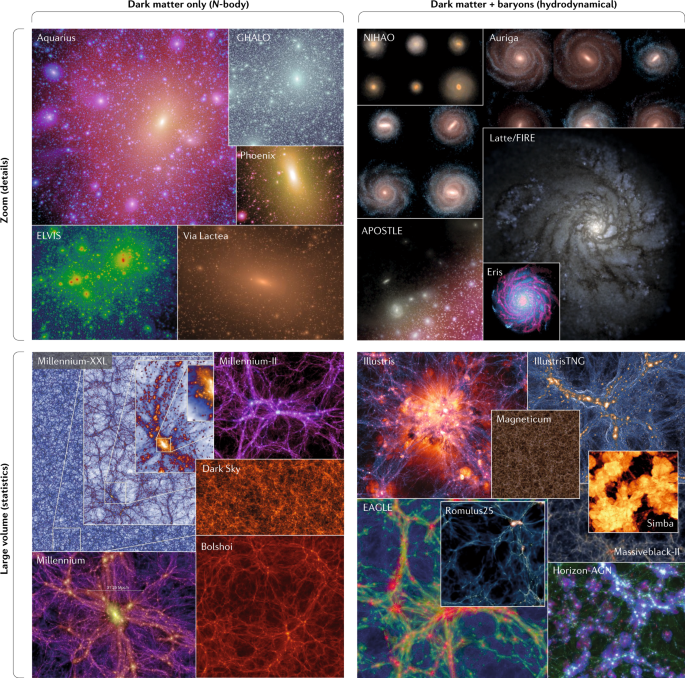
\includegraphics[scale=0.6]{img/cosmo-sims.png}
    \caption{The simulations are divided into large-volume
simulations that provide statistical samples of galaxies and zoom simulations that
resolve smaller scales in more detail. They are also divided in dark matter-only
simulations, such as N-body simulations, and dark matter plus baryons
simulations, such as hydrodynamical simulations. Dark matter-only simulations
have now converged on a wide range of predictions for the large-scale clustering
of dark matter and the dark matter distribution within gravitationally bound dark
matter halos. Recent hydrodynamical simulations reproduce galaxy populations
that agree remarkably well with observational data. However, many detailed
predictions of these simulations are still sensitive to the underlying
implementation of baryonic physics. }
    \label{fig:enter-label}
\end{figure}

To study the co-evolution of MBH and galaxies in a cosmological context, there are two kinds of approach - using cosmological hydrodynamical simulations and semi-analytical models. In cosmological simulations, the DM and barynic components od the universe are evolved starting from a set of initial conditions. These are in general computationally expensive compared to the other approach - SAM. SAMs generally follow through the baryonic evolution through a set of serious of differential equations. They usually involve the simplistic prescription of the physics but has an advantage of being computationally inexpensive and able to probe how the galaxy population is affected by targeted physical assumptions. Also, SAMs are unable to target the internal structure and evolution of galaxies which are important for modeling MBHs. Although cosmo sims can track this, many are unable to resolve the smaller scale physics that lies beyond the spatial resolutions of these sims. Hence, there are many ``zoom-in" simulations developed to probe smaller resolutions. To bridge this gap in large-volume simulations, subgrid models for the small scale physics needs to developed. 


\newpage

\section{Cosmological Simulations}

Cosmological simulations are developed for a specific volume box and there is a trade-off between the size of the volume and the mass and spatial resolution desired. The state of the art simulations are able to simulate $\sim$ [100 cMpc]$^3$ volume with kpc spatial resolutions. This \href{https://www.nature.com/articles/s42254-019-0127-2}{nature review } goes over the cutting edge cosmological simulations currently used in galaxy evolution research. The initial conditions of these simulations specify the the density perturbations imposed on the FLRW metric. The scale invariant quantum mechanical fluctuations of cosmic inflation is described by Gaussian functions described by the matter power spectrum $P(|k|)$. The matter power spectrum used to generate the simulations takes the form $A k^n |T(k)|^2$, where $|T(k)|$ is the transfer function linking the post-recombination density field with the primordial density function predicted by inflation.

\begin{mybox}[title={Initial conditions}]
Initial positions are definied as $\mathbf{x} = \mathbf{q} + D(t) \Psi $.\\
Intital velocities are defined as 
\begin{align}
    a(t) \dot{\mathbf{x}} &= a(t) \frac{d D(t)}{d t} \mathbf{\Psi}(q)\\
    &= a(t) H(t) \frac{d \ln{D}}{d \ln{a}} D(T) \mathbf{\Psi}(q)
\end{align}

where $D(t)$ is the linear growth factor, $a$ is the scale factor which is related to the redshift $z = \frac{1}{a}-1$ and $H
(t)$ is the Hubble parameter. The curl-free displacement field is defined by the linearized continuity equation

\begin{equation}
    \nabla \cdot \Psi = \frac{- \delta}{D(t)}
\end{equation}

where $\delta$ is the relative density fluctuation. Check \href{https://www.astro.rug.nl/~weygaert/tim1publication/lss2009/lss2009.linperturb.pdf}{these notes} for linear perturbation theory. 

\todo{Add this in the cosmology and GR theory notes.}

\end{mybox}
\subsection{Simulating dark matter \& baryons}
Dark Matter is the backbone of galaxies and they emerge as the centers of the dark matter over-densities - halos. They are described by the \href{https://web.physics.ucsb.edu/~mccann/notes/Virial.pdf}{ collision-less Boltzmann equation} coupled to Poisson's equation. Their evolution is described in an expanding universe described by the Friedmann equations which are derived from the field equations in GR. However, simulations employ Newtonian gravity as it provides a good approximation in the linear growth regime and non-linear structure evolution produces velocities are much below $c$. The Boltzmann equations are solved numerically using the N-body method. This requires us to calculate the gravitational forces of the N-body system which is a challenge as it requires solving either the integral or the differential form of the Poisson's equation.

\begin{mybox}[title=Modelling dark matter]

DM is described by the collision-less Boltzmann equation and N-body methods is used to solve it. 

\begin{equation}
    \label{eq:Boltzmann-collisonless}
    \frac{df}{dt} = \frac{\partial f}{\partial t} + \textbf{v} \frac{\partial f}{\partial \textbf{r}} - \frac{\partial \Phi}{\partial \textbf{r}} \frac{\partial f}{\partial \textbf{r}} = 0
\end{equation}

This describes the evolution of the phase-pace density or distribution function of DM $f(\textbf{r},\textbf{v},t)$ under the influence of the gravitational potential $\Phi$ which is solved via N-body methods.

\begin{equation}
    \label{eq:poisson-eqn}
    \nabla^2 \Phi = 4 \pi G \int f d \textbf{v}
\end{equation}
\todo{Add notes for the boltzmann equation in galaxy evolution notes.}

\end{mybox}

The earliest DM simulations studied the large scale distribution of DM. CDM simulations shod rhat the distribution is not completely homoheneous, nut they exhibit web-like structures: \textbf{voids, walls and filaments} which are quantified by halo mass function (HMF). The HMF is defined as the comoving number density of the dark matter halos as a function of their \href{https://en.wikipedia.org/wiki/Virial_mass}{virial mass} $M_{\rm vir}$ which is typically defined as $M_{200}$, the mass enclosed within a radius $r_{200}$ containiting the mean density 200 times the critical mass density of the universe. The virial 

\begin{equation}
    \rho(r < r_{\rm vir}) = \Delta_c \rho_c (t) = \Delta_c \frac{3 H^2(t)}{8 \pi G} \approx 200 \rho_c(t)
\end{equation}

A mathematical formulation of the HMF is given in \citet{Tinker_2008} which is based on the \citet{PS_1974} formalism. A detailed review of the HMF from DM simulations is given in  \citet{Jenkins_2001}. These studies showed that the low-mass end of the halo mass function has a power law slope close to -2 and the high-mass end is exponentially suppressed. 

In simulations, the DM halos are identified using \href{https://swift.strw.leidenuniv.nl/docs/FriendsOfFriends/algorithm_description.html}{friend-of-friends algorithm}. TWithin the collapsed and virialized DM halos identifies, these simulations have been effective at probing their structure. The DM distribution within halos is described by a near-universal spherically averaged density profile called the \textbf{\href{http://www.astro.yale.edu/vdbosch/jerusalem_lecture3.pdf}{Navarro-Frenk-White (NFW) profile}}. 

\begin{equation}
    \label{eq:NFW}
    \rho(r) = \frac{\rho_s}{\left(\frac{r}{r_s} \left(1 + \left(\frac{r}{r_s} \right)^2 \right)\right)}
\end{equation}

where $\rho_s$ and $r_s$ represents cracteristic density and transition radius respectively. The central slop of DM halos has been debated (\href{https://arxiv.org/pdf/0910.3538}{cusp-core problem}) and is affected by the baryonic physics. Recent simulations have shown found a slope shallower than -1, leading to a density profile with changing slope profile as a better choice. This is known as the \textbf{Einasto profile}:

\begin{equation}
    \label{eq: Einasto}
    \ln{\left(\frac{\rho(r)}{\rho_{-2}}\right)} = \frac{-2}{\alpha} \left[ \left( \frac{r}{r_{-2}} \right)^{\alpha} -1 \right]
\end{equation}

where $r_{-2}$ is the transition radius and the slope is defined by a power law. The concentration parameter $ c = r_{\rm vir}/r_s$ correlates with the mass of the halo $c \propto M^{- \delta}, \delta \approx 0.1$. Simulations showed that the dependence of halo concentration on things like the mass and initial fluctuation spectrum is all reflective of its dependence with the halo formation time \citep{Navarro_1997}. Lower mass halos formed earlier in time and hence have higher concentration, due to the higher density of the university at the time of formation. Halos within halos, called subhalos could be resolved as resolutions of these cosmo-sims increased. 



Although DM and dark energy dominate $\sim 95 \%$ of the energy density of the universe, the baryons are the visible component. Therefore simulating them is crucial for making predictions. The first baryons were gas - mainly composed of hydrogen and helium. Some of the gas eventually turned into stars during structure formation. Astrophysical gas in these simulations are described by inviscid ideal gases following \textbf{Euler equations}. The hydrodynamical equations can be discretized using numerical techniques that fall into three classes - Lagrangian, Eulerian and Lagrangian-Eulerian techniques. 


\begin{figure}[!htb]
    \centering
    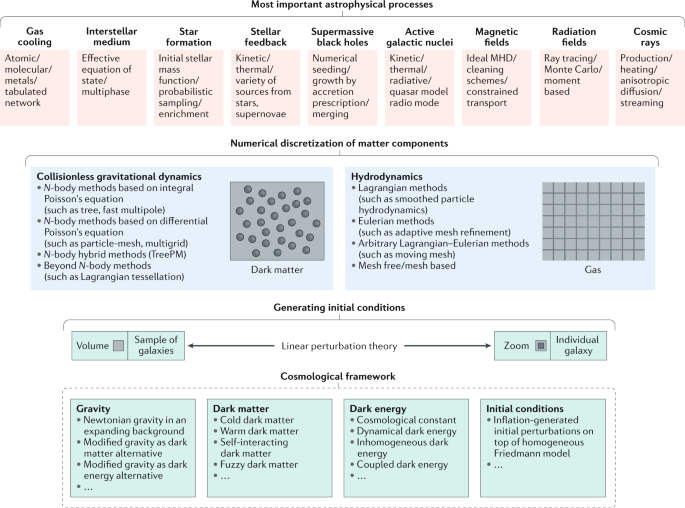
\includegraphics[width=0.8\linewidth]{img/sim-physics.png}
    \caption{These simulations are performed within a given
cosmological framework and start from specific initial conditions. The framework includes physical models for gravity,
dark matter, dark energy and the type of initial conditions. Two types of simulations are typically performed: either
large-volume simulations or zoom simulations. The evolution equations of the main matter components, dark matter
and gas, are discretized using different techniques and evolved forward in time. The dark matter component follows
the equations of collisionless gravitational dynamics that are in most cases solved through the N-body method using
different techniques to calculate the gravitational forces. The gas component of baryons is described through the
equations of hydrodynamics that are solved, for example, with Lagrangian or Eulerian methods. Various astrophysical
processes must also be considered to achieve a realistic galaxy population. Many of these are implemented through
effective subresolution models. MHD, magnetohydrodynamics; TreePM, tree + particle-mesh.}
    \label{fig:enter-label}
\end{figure}



\subsection{Baryon physics included}


\subsection{Illustris and IllustrisTNG}

The Illustris simulation suite is a set of cosmological, hydrodynamical simulations run using the {\tt AREPO}  code \citep{Springel_2010}. This code combines the advantages of smooth particle (SPH) (e.g. \citep{Gingold97, Lucy1997}) and an Eulerian-mesh-based approach (e.g. \citep{BERGER198964}). The highest resolution run, `Illustris-1'(referred in this work simply as Illustris), is a cosmological box of side $L_{\text{box}} = 75 h^{-1}$ Mpc. This simulation has a DM resolution of $6.3 \times 10^6 M_{\odot}$ and a baryonic mass resolution of $1,2 \times 10^6 M_{\odot}$ and runs from $z=137$ to $z=0$. The simulations assume a WMPA9 cosmology \citep{Hinshaw_2013} with parameters $\Omega_m = 0.2865$, $\Omega_{\Lambda} = 0.7135, \sigma_{8} = 0.820$, and $H_{0} = 70.4$ \kms Mpc$^{-1}$.


\subsubsection{Seeding models and the BRAHMA simulation}


\subsubsection{Other important cosmo-sims}

\subsubsection{ASTRID}
\subsubsection{NewHorizon}

\subsubsection{Romulus}



      
\section{Semi-Analytical Models}

The Illustris cosmological simulation



\chapter{MBH formation}


\chapter{MBH binary dynamics}


\chapter{MBH accretion}

\chapter{Gravitational waves from MBHBs}


\bibliographystyle{unsrtnat}
\bibliography{references}
\end{document}
